% =========================================================================
% Beamer deck: From IMP restraints to BlackJAX SMC sampling
% Compile with:  pdflatex  imp_to_blackjax.tex   (twice)
% Falls back to default theme if `metropolis` is not installed.
% =========================================================================
\documentclass[10pt,aspectratio=169]{beamer}

% -- theme -----------------------------------------------------------------
\IfFileExists{beamerthememetropolis.sty}{%
    \usetheme{metropolis}%
}{%
    \usetheme{Boadilla}%
    \usecolortheme{seahorse}%
}

% -- packages --------------------------------------------------------------
\usepackage[T1]{fontenc}
\IfFileExists{lmodern.sty}{\usepackage{lmodern}}{}
\usepackage{amsmath, amssymb}
\usepackage{listings}
\usepackage{xcolor}
\usepackage{tikz}
\usetikzlibrary{arrows.meta, positioning, shapes.geometric, fit, backgrounds}

% -- listings style for Python --------------------------------------------
\definecolor{codebg}{RGB}{246,246,248}
\definecolor{codecmt}{RGB}{100,110,120}
\definecolor{codekw}{RGB}{160,40,140}
\definecolor{codestr}{RGB}{40,120,60}
\lstdefinestyle{py}{%
    language=Python,
    basicstyle=\ttfamily\footnotesize,
    backgroundcolor=\color{codebg},
    keywordstyle=\color{codekw}\bfseries,
    commentstyle=\color{codecmt}\itshape,
    stringstyle=\color{codestr},
    showstringspaces=false,
    breaklines=true,
    columns=fullflexible,
    keepspaces=true,
    aboveskip=4pt, belowskip=4pt,
}

% -- metadata --------------------------------------------------------------
\title{From IMP restraints to BlackJAX SMC sampling}
\subtitle{A two-stage bridge: C\texttt{++} scores \(\to\) JAX, structured model \(\to\) flat vector}
\author{Sree Ganesh Balasubramani}
\institute{Echeverria \& \v{S}ali groups, QBI, UCSF}
\date{}

% =========================================================================
\begin{document}

\maketitle

% ==================================================================  1  ===
\begin{frame}{The problem: two representations, one sampler}

\textbf{IMP-side reality.}
Integrative restraints are implemented in C\texttt{++} and operate on a
\emph{structured} model: rigid bodies with translations and quaternions,
slaved member particles with internal coordinates, and free beads with
plain Cartesian \texttt{xyz}.

\medskip
\textbf{BlackJAX-side requirement.}
SMC kernels in
\texttt{blackjax.smc.base} expect a flat \((n_\text{particles},\, n_\text{dims})\)
array of particles and a pure-JAX scalar function
\(\log\pi(x)\) that is both \texttt{jit}-able and \texttt{vmap}-able.

\medskip
\textbf{Bridge.}
Two layers are introduced. In \textbf{Stage 1 (scoring)}, IMP restraints are
exposed as pure JAX functions over a structured model dictionary, via SWIG
\texttt{\%extend} blocks. In \textbf{Stage 2 (geometry)}, the structured
model is mapped onto a flat parameter vector, with rigid-body slaves
propagated internally so the sampler never sees them.

\begin{center}
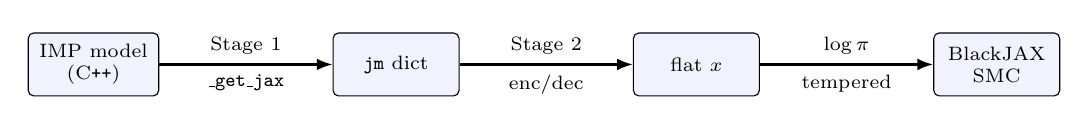
\begin{tikzpicture}[
    node distance=4mm and 22mm,
    every node/.style={font=\scriptsize},
    box/.style={draw, rounded corners=2pt, align=center, inner sep=4pt,
                minimum height=8mm, minimum width=16mm, fill=blue!5},
    arr/.style={-{Latex[length=2mm]}, thick},
]
\node[box]                        (imp)   {IMP model\\(C\texttt{++})};
\node[box, right=of imp]          (jm)    {\texttt{jm} dict};
\node[box, right=of jm]           (flat)  {flat \(x\)};
\node[box, right=of flat]         (smc)   {BlackJAX\\SMC};

\draw[arr] (imp)  -- node[above]{Stage 1}   node[below]{\scriptsize\texttt{\_get\_jax}}  (jm);
\draw[arr] (jm)   -- node[above]{Stage 2}   node[below]{\scriptsize enc/dec}             (flat);
\draw[arr] (flat) -- node[above]{$\log\pi$} node[below]{\scriptsize tempered}            (smc);
\end{tikzpicture}
\end{center}

\end{frame}

% ==================================================================  2  ===
\begin{frame}[fragile]{Stage 1: IMP restraints \(\to\) JAX scoring}

\textbf{Mechanism.}
Each restraint, unary function, and pair score is decorated, via SWIG
\texttt{\%extend} blocks, with a \texttt{\_get\_jax()} method that returns
an equivalent pure-JAX implementation. The aggregate
\texttt{RestraintsScoringFunction} sums them and returns a
\texttt{JAXRestraintInfo} object.

\begin{lstlisting}[style=py]
%extend IMP::core::HarmonicDistancePairScore {
  %pythoncode %{
    def _get_jax(self, m, indexes):
        def jax_harmonic(jm, d, k):
            xyzs = jm['xyz'][indexes]
            diff = xyzs[:,0] - xyzs[:,1]
            drs  = jnp.linalg.norm(diff, axis=1)
            return 0.5 * k * (d - drs)**2
        ...
  %}
}
\end{lstlisting}

\textbf{What is obtained.}
A single callable \(\,s_\text{JAX}:\, \texttt{jm} \mapsto \mathbb{R}\,\) is
produced such that
\(s_\text{JAX}(\texttt{jm}) \approx s_\text{C\texttt{++}}(\text{IMP model})\),
and is now \texttt{jit}-compilable, \texttt{vmap}-compatible across
particle batches, and (if all terms are differentiable) amenable to
\texttt{jax.grad} for HMC kernels.

\end{frame}

% ==================================================================  3  ===
\begin{frame}[fragile]{The structured JAX model \texttt{jm}}

\textbf{Layout of} \texttt{jm}\textbf{, the input to} \(s_\text{JAX}\)\textbf{.}
The dictionary carries all per-particle quantities that any IMP-side
restraint may read:
\texttt{jm['xyz']} of shape \((N,3)\) holds global Cartesian coordinates;
\texttt{jm['r']} of shape \((N,)\) holds radii; and
\texttt{jm['rigid\_bodies']} is an \texttt{\_AllRigidBodies} dataclass
carrying rigid-body topology and pose.

\textbf{Rigid-body sub-structure.}
\begin{lstlisting}[style=py]
@register_dataclass
class _AllRigidBodies:
    intcoord   : jnp.ndarray   # (N, 3) member-local coordinates
    quaternion : jnp.ndarray   # (n_rb, 4) reference-frame rotations
    bodies     : list[_RigidBody]   # topology, parent-child pointers
\end{lstlisting}

\textbf{Slave propagation.}
For each body, \texttt{body.update\_members(jm)} recomputes the global
\texttt{xyz} of its non-root members from the parent's
(translation, quaternion) and the cached internal coordinates. Nested
bodies are handled by iterating over \texttt{bodies} in parents-first
order, the IMP default. The sampler, however, operates on flat
\(\mathbb{R}^{n_\text{dims}}\) vectors and cannot consume a heterogeneous
dictionary, nor enforce unit-norm quaternions -- a flattening layer is
required.

\end{frame}

% ==================================================================  4  ===
\begin{frame}[fragile]{Stage 2: \texttt{IMPDOFSpace} -- flat \(\leftrightarrow\) structured}

\textbf{Flat-vector layout.}
Only the truly free degrees of freedom are exposed; slaved members are
recomputed inside \texttt{decode}. With \(n_\text{rb}\) rigid bodies and
\(n_\text{fb}\) flexible beads:
\[
    x \;=\; \bigl[\,
        \underbrace{\mathbf{t}_{1:n_\text{rb}}}_{3 n_\text{rb}}\,\big|\,
        \underbrace{\mathbf{q}_{1:n_\text{rb}}}_{4 n_\text{rb}}\,\big|\,
        \underbrace{\mathbf{r}_{1:n_\text{fb}}}_{3 n_\text{fb}}
    \,\bigr]
    \;\in\;\mathbb{R}^{n_\text{dims}},
    \qquad n_\text{dims} \,=\, 7\,n_\text{rb} + 3\,n_\text{fb}.
\]

\textbf{Encoding.}
\(\texttt{encode}(\texttt{jm})\) reads the translations from
\(\texttt{jm['xyz']}\), the quaternions from
\(\texttt{jm['rigid\_bodies'].quaternion}\), and the flexible-bead
positions, and concatenates them.

\textbf{Decoding.}
\(\texttt{decode}(x)\) is the non-trivial direction:
\begin{enumerate}
    \item Quaternions are renormalised, \(\mathbf{q}_i \leftarrow \mathbf{q}_i / \|\mathbf{q}_i\|\),
          so that Gaussian RMH/HMC proposals always project onto~\(S^3\).
    \item A shallow copy of \texttt{template\_jm} is patched in place using
          \texttt{xyz.at[\dots].set(\dots)} and
          \texttt{dataclasses.replace} -- the template itself is never
          mutated, so multiple particles can decode in parallel under
          \texttt{vmap}.
    \item \texttt{body.update\_members(jm)} is invoked for every rigid
          body, restoring consistency between the new pose and all slaved
          members.
\end{enumerate}

\end{frame}

% ==================================================================  5  ===
\begin{frame}[fragile]{Stage 2b: \texttt{IMPSMCAdapter} \(+\) BlackJAX base SMC}

\textbf{Densities exposed to the sampler.}
The adapter composes \texttt{decode} with the JAX score function and
adds soft regularisers:
\begin{align*}
    \log\,p_\text{lik}(x)   &= -\,s_\text{JAX}\bigl(\,\texttt{decode}(x)\,\bigr)\,/\,k_BT, \\
    \log\,p_\text{prior}(x) &= -\tfrac{1}{2\sigma_\text{box}^2}\!\!\sum_i \!\max(|x_i| - L, 0)^2
                              -\tfrac{1}{2\sigma_q^2}\!\!\sum_j(\|\mathbf{q}_j\|-1)^2, \\
    \log\,\pi(x)            &= \log\,p_\text{prior}(x) + \log\,p_\text{lik}(x).
\end{align*}

\textbf{Tempered SMC loop} (\texttt{run\_base\_smc\_rmh}).
A schedule \(0 = \lambda_0 < \dots < \lambda_T = 1\) is fixed in advance
(linear, geometric, or sigmoid), targeting
\(\pi_t(x) \propto p_\text{prior}(x)\,p_\text{lik}(x)^{\lambda_t}\) at
step \(t\). Each step \textbf{reweights} particles by
\(w_t(x) = (\lambda_t - \lambda_{t-1})\,\log p_\text{lik}(x)\),
\textbf{resamples} systematically, and \textbf{mutates} via
\(n_\text{mcmc}\) RMH (or HMC) sweeps targeting \(\pi_t\), batched across
particles by \texttt{vmap} and memory-bounded by \texttt{batched\_vmap}.
The final \texttt{state.particles} of shape
\((n_\text{particles},\, n_\text{dims})\) is decoded row by row via
\texttt{adapter.decode\_xyz} to recover full \((N,3)\) coordinate sets
for RMF3 writing or downstream analysis.

\end{frame}

\end{document}